\documentclass{standalone}
\usepackage{standalone}

\begin{document}
\section{Logistic Regression}
When the dependent variable is categorical, then logistic regression is one of the most appropriate regression model. Logistic regression is a binary classifier, but multiple classification is possible using one vs. all model. 
If a data set D = {(x,y) : x $\epsilon$ X , y $\epsilon$ Y} where X is the independent variables and Y is the set of category. The hypothesis function h $\theta$(x) is given below which is a sigmoid function, 

\begin{center}
	\makebox h\textsubscript{ $ \theta $}{(x)} = $ \frac {1}{1+e^{-\theta^{T}X}} $ \\
\end{center}

Using this hypothesis function a curved line is drawn which is used to classify the data. To derive the coefficients a cost function J($\theta$) is used. The value of J($\theta$) is shown in following equation,\\

%J($\theta$) = $ \frac{1}{m}\sum_{i=1}^{m}[y\textsubscript{i}\log h\textsubscript{\theta}{(x\textsubscript{i})}+{(1-y\textsubscript{i})}\log (1-h\textsubscript{\theta}{(x\textsubscript{i})})]  $ \\
\begin{center}
	\makebox J(\theta) = -\frac{1}{m}\sum_{i=1}^{m}[y\textsubscript{i} \log h{$\textsubscript{\theta}$}{(x\textsubscript{i})}+{(1-y\textsubscript{i})}\log (1-h{$\textsubscript{\theta}$}{(x\textsubscript{i})})]\\
\end{center}
\begin{figure}[h]
				\centering
				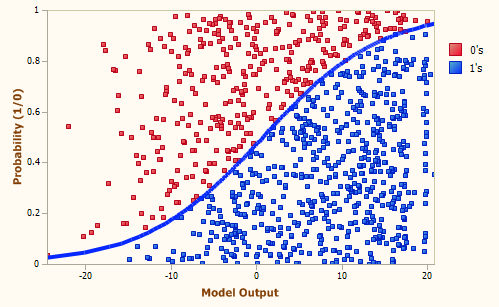
\includegraphics[scale=0.8]{./img/lor}
				\caption{Basic Logistic Regression} \label{fig:mapComp}
\end{figure}

After minimizing the cost function, the values of the coefficients are derived. The following equation is used to update the values of $\theta$, 

\begin{center}
	\makebox  $\theta$\textsubscript{j} = $\theta$\textsubscript{j}- $\frac{1}{m}$ \sum_{i=1}^{m} ( h\textsubscript{j}(x\textsubscript{i})- y\textsubscript{i})x\textsubscript{j}  \\
\end{center}


\end{document}